% !TeX spellcheck = en_GB
\documentclass[../summary.tex]{subfiles}

\begin{document}
	
	\section{Climate}
		\stepcounter{subsection}
		\subsection{Climate trends and causes}
			\subsubsection{Climate change over geological cycles}
				We know climate change is partly a natural phenomenon because of the research done with Antarctic ice. Figure \ref{fig:1-antarctic-ice-records} clearly shows a natural cycle in temperatures over the last 800,000 years. Other evidence pointing to this conclusion can be found in landscapes which have been altered by moving glacial ice.
				\begin{figure}[h]
					\centering
					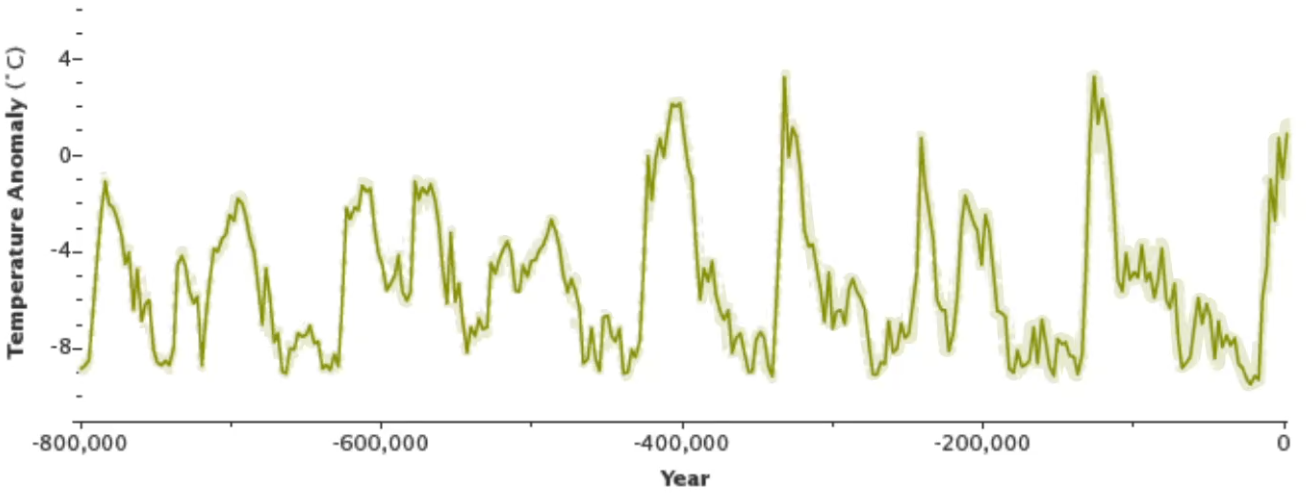
\includegraphics[width=0.7\linewidth]{../images/1-antarctic-ice-records.png}
					\caption{Antarctic ice records}
					\label{fig:1-antarctic-ice-records}
				\end{figure}
			
			\subsubsection{Causes of climate change}
				There are a few factors which cause the change in climate on earth:
				\begin{itemize}
					\item Variations in the earth's orbit around the sun (eccentricity)
					\item The axis of the Earth from pole to pole is tilted compared to this plane of movements, this is time dependent (obliquity)
					\item Precession of the Earth. 
				\end{itemize}
				Of these especially obliquity is important. It can lead to very hot summers and very cold winters without a lot of snowfall. This leads to a shrinkage in the ice coverage of the Earth which leads to ever warmer temperatures. This feedback loop amplifies itself (albedo feedback). Another factor is the physical place of land mass. If it is close to the poles, ice can easily form and reflect heat back into space. Volcanic explosions are known to have an influence as well due to their tendency to throw light blocking particles in the atmosphere. Lastly the activity of the sun itself plays a role in the climate of the earth. \\
				\\
				Us humans have had an impact since the industrial revolution by throwing tiny particles in the air due to burning fossil fuels, cooling the earth. This effect is overshadowed by the fact that we emit a lot of greenhouse gasses whilst we burn the same fossil fuels. An illustration of our impact on $CO_2$ levels can be seen in figure \ref{fig:1-co2-history}.
				\begin{figure}[h]
					\centering
					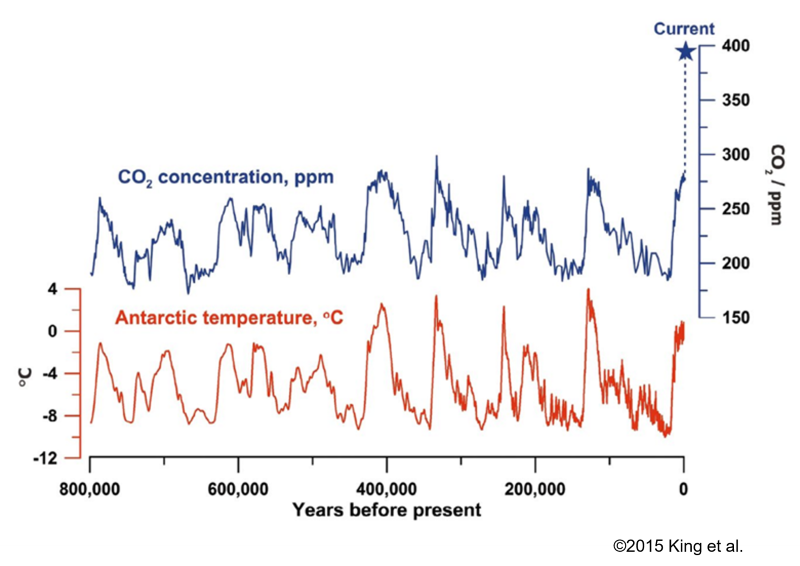
\includegraphics[width=0.7\linewidth]{../images/1-co2-history.png}
					\caption{Historic $CO_2$ records}
					\label{fig:1-co2-history}
				\end{figure}
				
			\newpage
			\subsubsection{Human cause}
				Global temperatures have increased by 1.1 degrees Celsius since industrialization. There are five lines of evidence that our greenhouse gas emission is responsible for this:
				\begin{enumerate}
					\item We see that our activities with fossil fuel and cement produces about 9Gt of carbon per year, whilst the natural rate is only 0.9Gt per year. Luckily for us, the earth absorbs about 5.5Gt per year back into itself, otherwise $CO_2$ levels would be double of what they are right now. 
					\item We also look at the isotopic ratio between C13 and C12 carbon. The gradual lowering of this ratio suggests a lot of plant derived carbon sources (fossil fuels) have been dumped in the atmosphere. 
					\item The physical mechanism by which greenhouse gasses prevent infra-red radiation from escaping our atmosphere has been proved already in 1850.
					\item Climate models where factors can be individually adjusted also show a large effect of our activity.
					\item Radiative forcing is what happens when the amount of energy that enters the Earth's atmosphere is different from what leaves it. This, again, is influenced by greenhouse gasses.
				\end{enumerate}
			
			\subsubsection{Radiative forcing}
				As discussed in the previous section, radiative forcing has an impact on our climate, but how does it work? The only way in which the earth can exchange energy is through radiation interactions with space. This is depicted in figure \ref{fig:1-radiation-exchange}.  In the end, about 31\% of the solar radiation is reflected. This yields a net solar radiation of about 235 watts per square meter. In reality this net radiation is counteracted by the natural infra-red radiation of earth, balancing the entire system. \\
				\\
				By emitting too many greenhouse gasses, we have brought this balance to an end, resulting in a net increase of energy. To investigate the forcing effect we have, we can look at a concept called radiative forcing. This is a very important concept in the whole climate research and also very important for policy implications because with this metric, we can estimate the effect of different forcing factors.\\
				
				\begin{figure}[h]
					\centering
					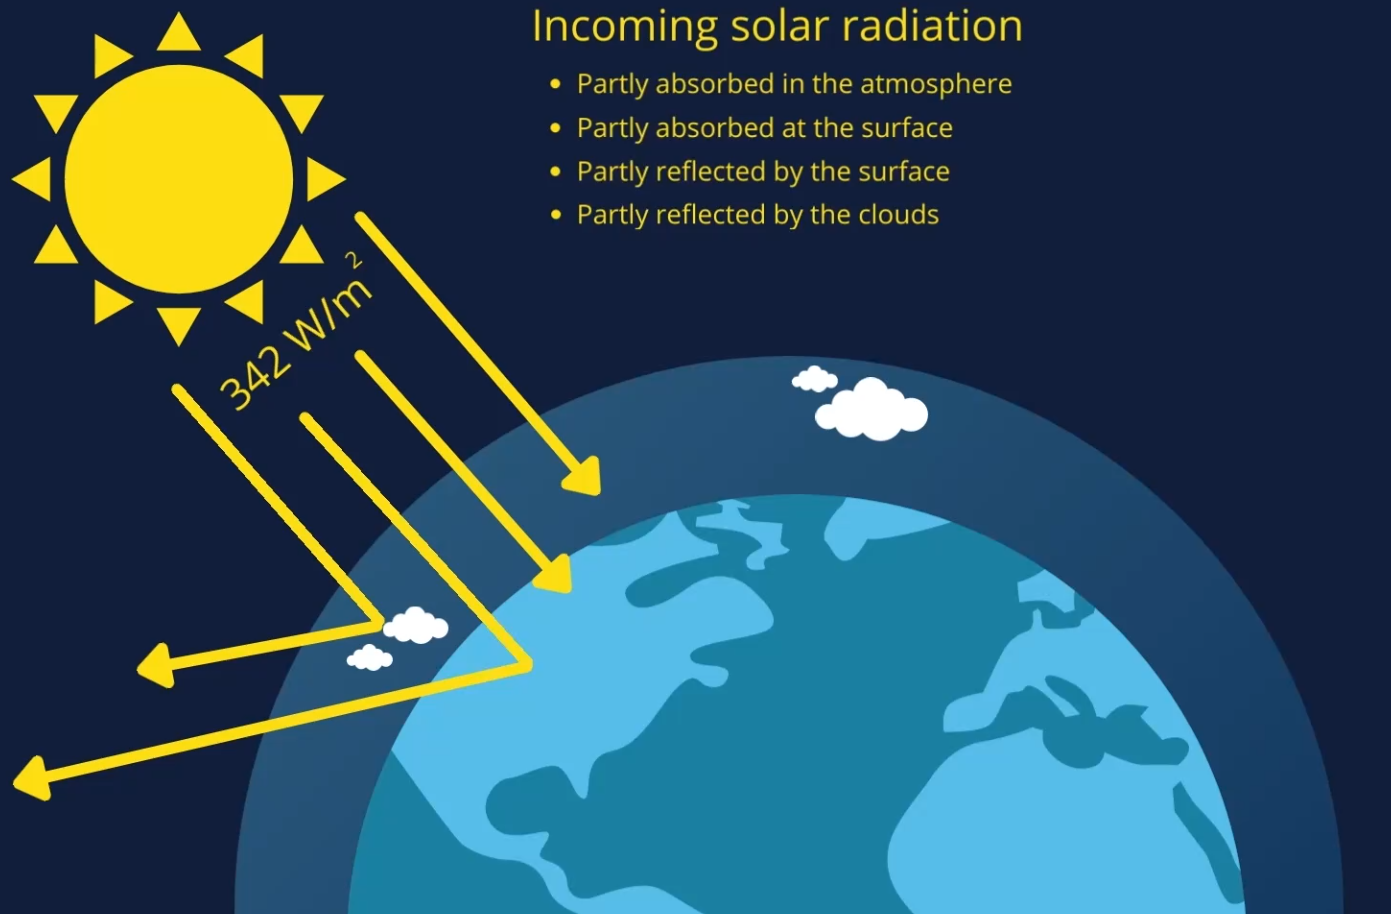
\includegraphics[width=0.7\linewidth]{../images/1-radiation-exchange.png}
					\caption{Earth's radiation exchange}
					\label{fig:1-radiation-exchange}
				\end{figure}
				\newpage
				So when we sum everything up over the time period 1750 till now, then we can also look at the average radiative forcing over that time period. The radiative forcing by carbon dioxide is the largest contributor - so that's why we talk about CO2 a lot when we are talking about climate change - namely 2.16 watts per square meter. Other well-mixed gasses also play an important role, so they also cause a positive radiative forcing. Ozone as well.
				% We moeten potentieel wel nog is zien naar deze sectie want ik had het echt zwaar gehad.
				
		\subsection{Climate targets and pathways}
			\subsubsection{International agreements}
				A very important milestone in the climate negotiation is the Paris Agreement of 2015. The goal of this convention is to stabilize greenhouse gas concentrations at a level that would prevent dangerous anthropogenic interference with the climate system by keeping the maximum warming under 2 --preferably 1.5-- degrees Celsius. This target is based on scientific research by the entire climate community worldwide called the Intergovernmental Panel on Climate Change (IPCC).\\
				\\
				The IPCC bases their recommendations on hundreds of papers and years of research of how the emission of greenhouse-gasses impacts the Earth. Since there are so many aspects to climate change, they have formed five subdivisions:
				\begin{description}
					\item[Geographic] Preserving coral reefs, Arctic and indigenous people, mountain glaciers and biodiversity hotspots.
					\item[Weahter] Extremes like heat waves, heavy rains, droughts, wildfires, coastal flooding.
					\item[People] Concern for impacts that disproportionately affect particular groups.
					\item[Monetary damage]  Global scale degradation, loss of ecosystems and biodiversity on a global scale could lead to global damages and making the world more difficult to live in
					\item[Climate system] Concern for the large, abrupt and sometimes irreversible changes in the system. These are called tipping points as well.
				\end{description} 
			
			\newpage
			\subsubsection{Carbon budget}
				To reach our goal of keeping climate change to a minimum, we need to gauge how much we need to achieve for that. For this reason, the carbon budged was introduced: it is a measure of how much $CO_2$ we can still emit without going over the limit. Part of this budged has already been spent because we calculate the budged from the start of our industrialization. \\
				\\
				Calculating this figure is not easy, but we can take some short-cuts: temperature is linearly proportional to $CO_2$ emissions. This is clearly shown in figure \ref{fig:1-co2-temp}. This of course isn't conclusive evidence about the relationship and thus the prediction of our carbon budged can be wrong. A probability of 66\% (the very likely range) has been chosen, meaning that the carbon budget is defined in a way that we have a 66\% chance to stay within the temperature targets that have been defined by the Paris Agreement.
				\begin{figure}[h]
					\centering
					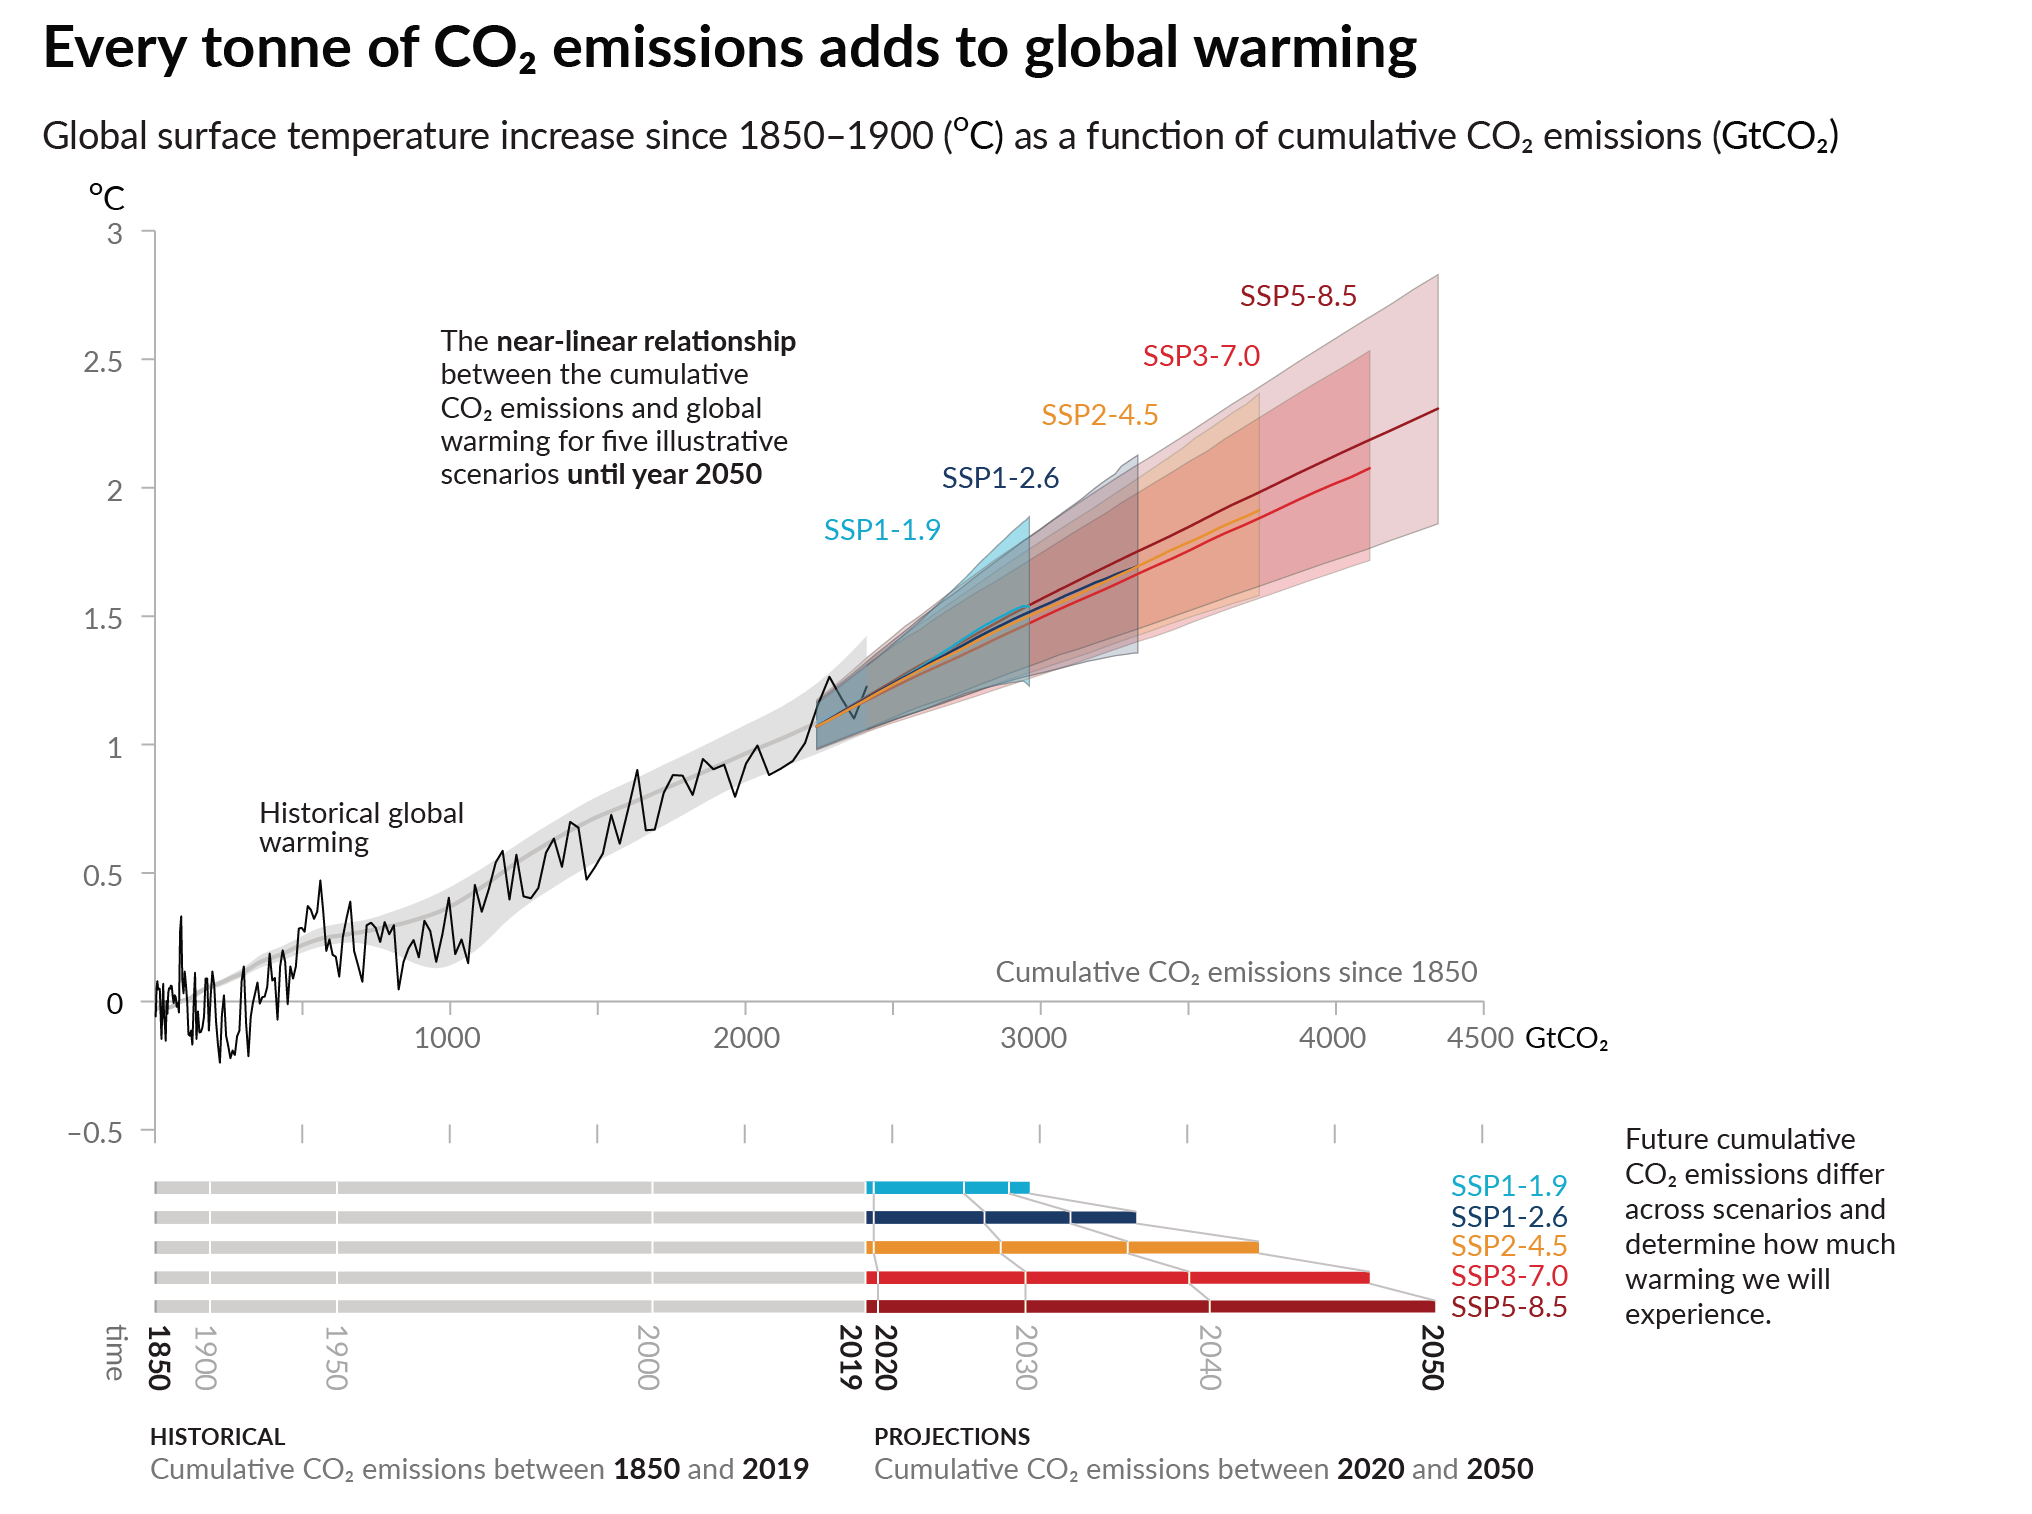
\includegraphics[width=0.7\linewidth]{../images/1-co2-temp.png}
					\caption{Relationship between $CO_2$ and temperature}
					\label{fig:1-co2-temp}
				\end{figure}
				% Nog een deel over andere gassen er uit gelaten omdat het er uit ziet als een sidenote
				
			\subsubsection{Pathways}
				Because the exact time of emission is almost irrelevant, the IPCC has found four different pathways to reducing emissions. There are essentially 2 types: Strong reductions at the start with lower effort later down the line, and low effort now with (almost unrealistic) reductions later. They also rely very much on negative emissions, meaning that carbon is stored either in biosystems or in engineering systems\\
				\\
				All pathways rely heavily on the reduction of fossil fuels. We also will have to do some land management: agriculture, forestry and other land use (AFOLU). Thirdly we can use bioenergy with carbon capture and storage (BECCS). The first two pathways mainly rely on the reduction of fossil fuels, the fourth pathway makes heavy use of BECCS and the third pathway combines both strategies. \\
				\\
				If we look at our efforts to reduce our $CO_2$ use by looking at the Emission Gap report, we see that our policy has had an impact on our emissions. However, to conform with the Paris Agreement by 2023 we still have a gap of about 12Gt to fill. % Bijna even veel dus als die hun dikke moeder
		
		\subsection{Climate mitigation}
			\subsubsection{What can I do?}
				An important resource of information is from the so-called drawdown project. Drawdown is the point in the future when levels of greenhouse gases in the atmosphere stop climbing and start to steadily decline. The drawdown project is the world's leading resource for climate solutions. Drawdown lists solutions based on effectiveness. So they estimate for a certain time horizon, in this case from 2020 to 2050, how much of the emission is either reduced or sequestered. \\
				\\
				For example, by reducing food waste to an absolute minimum we can save about 90Gt of emissions which is equal to about 2 years of emissions. Switching to plant rich diets would also help enormously in reducing the impact of agriculture and food on the climate. Other important changes are along the lines of managing refrigerants better, increasing forest coverage, transitioning to clean energy... .
				
			\subsubsection{Individual action} 
				There are four main ways to help fight climate change as an individual:
				\begin{enumerate}
					\item By using your democratic right, you can vote for political parties who take climate seriously. You can also participate in climate marches and activism to keep political pressure high. 
					\item Reducing your own carbon footprint: you can do this by changing habits such as diet, energy use, transportation choices... . The most effective starting point here is informing yourself. 
					\item Planet friendly investments by opting out of funds investing in fossil fuels. You can investigate in ethical banks and so on. Also inform yourself there
					\item Support an up scaling of the transition. If you can spread these ways to fight climate change and motivate others to do the same, then together we can do it
				\end{enumerate}
				
		\subsection{What can we expect for the future}
			\subsubsection{Climate scenarios}
				Running complete simulations of a possible future is expensive and difficult, that is why we introduced  representative concentration pathways or RPCs. They are labelled according to their radiative forcing: RPC 8.5 is 8.5 watts per square meter, RPC 5 is 5 watts per square meter... . \\
				\\
				Using RPCs we can make simpler models which reflect global warming. For example RPC 1.9 will get us to reaching our goals set on the Paris Agreement, while RPC 2.6 will probably lead to global warming by the end of this century. RPC 8.5 represents no change in climate policy and will have a large impact on our way of living. \\
				\\
				Looking at the impact of this warming, we see that the poles of the earth will heat the most. There is also a disproportionate heating effect between land and water. This is because it takes a huge amount of energy to heat water compared to heating land. Wet regions will get even wetter and dry regions will get even dryer. 
	
\end{document}